\chapter[Genetic Modification, Cloning, and Synthetic Biology]{Genetic Modification,\protect\\ Cloning, and Synthetic Biology}

\begin{kaichang}
Imagine two things: a golden Hawaiian papaya in a fruit shop, cut to reveal sweet, soft, juicy orange-red flesh; and ornamental fish glowing green under violet light, like swimming neon tubes.

What connects them? Both are \textbf{living organisms with deliberately rewritten DNA}. The papaya contains a short viral gene; the fish contain a jellyfish gene for a fluorescent protein.

Guess two things. Could the viral gene enter your body when you eat the papaya? Could releasing the fish destroy a river? Write down your intuition. By the chapter's end, you will see that ``genetically modified'' alone answers neither: each product requires its own questions, investigation, and assessment.
\end{kaichang}

\section{Ten Thousand Years of Rewriting Life}

Before high technology, look at fields and observable phenomena.

Modern maize has large ears and full kernels. Its wild Mexican ancestor, teosinte, had ears only a little finger long with a dozen or so hard seed cases. No miracle separated grass from maize. For millennia, farmers repeatedly \textbf{saved seeds from the plants they liked best and planted them next year}.

Consider fruit markets. Seedless bananas have three chromosome sets that pair chaotically, preventing normal seeds; the plants are cloned through cuttings. Large cultivated strawberries have eight chromosome sets, while woodland strawberries have two. Chihuahuas and Great Danes hardly resemble one species, yet both descend from wolves through over ten thousand years of selective breeding.

The lesson is that \textbf{traits can be rewritten, and humans have long done so}. Ancient farmers knew nothing of DNA, only that choosing, saving, and planting shifted the next generation toward their preferences. Their raw material was naturally occurring individual variation.

Another route is more forceful. Limited natural variation led twentieth-century breeders to generate more by irradiating seeds with gamma rays or applying chemicals, increasing DNA-copying errors and then selecting one useful plant among thousands with unknown changes. More than three thousand crop varieties worldwide arose through mutation breeding. Many rice, barley, and grapefruit ancestors passed through irradiation chambers. Interestingly, radically altered genomes in these varieties rarely provoke fear of ``mutant food.'' Revisit that contrast after reading the chapter.

\begin{shiyan}
\textbf{Observe Breeding's Raw Material: Variation.} Materials: two small handfuls of mung beans from one packet, two shallow dishes, water, and a ruler. Soak overnight, spread on damp paper towels, and place both dishes under matching light and temperature. Number each bean and record germination time and shoot length daily for a week. Which germinates first? How different are lengths after a week? Sort lengths and draw a simple distribution. Safety reminder: use clean water only, do not drink water that soaked raw beans, and wash afterward. Even with nearly identical genetic backgrounds, beans perform differently; mixing varieties would increase differences. Breeding's secret is selection on this distribution of variation.
\end{shiyan}

\textbf{Translator safety note:} Treat these sprouts as experimental material, not food, and discard them afterward. Harmful bacteria can multiply during sprouting even under apparently clean home conditions. See \href{https://www.fda.gov/food/buy-store-serve-safe-food/selecting-and-serving-produce-safely}{FDA sprout-safety guidance}.

\section{Zooming In: What Is Being Rewritten?}

Observation tells us traits change. At the particle level, what changes?

Recall the causal chain: DNA specifies proteins, proteins work in cells, and cells' collective behavior produces visible traits. Rewriting life ultimately means \textbf{changing DNA sequence}. Methods differ in how, how much, and how precisely.

Chapter 82 introduced restriction-enzyme scissors, ligase glue, plasmid couriers, and CRISPR's guided text editor. Chapter 83 showed them making bacterial insulin and teaching immune cells to attack cancer. Here we move to fields, farms, and fermenters and ask what happens after the change.

\section{Four Strategies Compared}

At the rule level, the debated terms breeding, genetic modification, and gene editing describe four DNA-rewriting strategies:

\begin{table}[htbp]
\centering
\small
\begin{tabular}{@{}p{2.6cm}p{4.6cm}p{2.6cm}p{3.2cm}@{}}
\toprule
Method & DNA change & Directed? & Typical example \\
\midrule
Conventional crossbreeding & Recombines both parents' whole genomes, followed by selection & Undirected; reshuffles tens of thousands of genes & Hybrid rice, dog breeds \\
Mutation breeding & Radiation or chemicals generate random mutations, then selection & Undirected, wholly random & Mutant barley, space-bred peppers \\
Transgenesis & Molecular tools insert one or two specific foreign genes & Directed introduction of known genes & Insect-resistant cotton, virus-resistant papaya \\
Gene editing & Changes a few bases at a specified genomic site & Most directed, but off-target effects possible & Disease-resistant wheat, nutrient-rich tomatoes \\
\bottomrule
\end{tabular}
\caption{Four DNA-rewriting approaches. The last column gives methods' examples, not automatic labels of safety or danger.}
\end{table}

Notice the counterintuitive point: conventional and mutation breeding \textbf{reshuffle the whole genome}, without checking every affected gene, while transgenesis and editing change only one or two precisely located genes. Ranking risk solely by change size could reverse popular expectations.

\begin{qiaoliang}
Common chemical mutagens can leave \textbf{thousands of point mutations} in a rice plant. Most remain unmapped and unexplained while breeders select good growth, letting the other mutations hitchhike to the table. A typical transgenic procedure introduces one or two sequenced, functionally studied genes. For comparison, every newborn carries roughly 60--100 mutations absent from the parents, copying mistakes during sperm and egg formation. A completely natural, never-mutated genome does not exist. This does not make change quantity irrelevant; it means \textbf{risk depends on what the changes produce, not merely whether changes occurred}. That leads to our central boundary.
\end{qiaoliang}

\section{Assess Products, Not Technology Labels}

Remember the chapter's most important sentence: \textbf{each product's traits and risks require individual assessment, not judgment from labels such as genetically modified or natural}.

Ask three questions:

\begin{itemize}[itemsep=2pt]
\item \textbf{What was introduced or changed?} What protein does it produce, and is that protein toxic or allergenic? Bt cotton carries a Bacillus thuringiensis gene whose protein binds receptors in particular insect guts, absent from human guts. Human exposure to Bt proteins predates engineered crops; organic farming has sprayed the bacterium as a biological pesticide for decades. Bt cotton greatly reduced chemical insecticide use and allowed beneficial insects such as ladybirds to recover. Yet pests evolve: repeated reliance on one method selects resistant bollworms, as Part Ten explained. Refuges of ordinary cotton retain susceptible insects that breed and dilute resistance. Even successful products require ongoing management.
\item \textbf{How much is produced, and where does it go?} Dose determines toxicity, Chapter 35's familiar rule. Does expression occur in fruit or roots? Could pollen carry it to weeds? Herbicide resistance reaching related weeds can create so-called superweeds, a real ecological issue requiring field isolation and management, not declarations of absolute safety.
\item \textbf{Is the resulting trait worthwhile?} Golden Rice adds two genes enabling endosperm production of $\beta$-carotene, a vitamin A precursor, for deficiency-affected regions. More than twenty years of safety evaluation and debate preceded cultivation approval in a few countries. By contrast, the first engineered food, delayed-ripening Flavr Savr tomato, had no safety failure but failed commercially through taste and costs. \textbf{Safety and success are different questions, both requiring evidence.}
\end{itemize}

\begin{zhengju}
How did scientists establish engineered papaya's efficacy and evaluate its safety individually? In 1992, papaya ringspot virus reached Hawaii's main production area. Spread by aphids, it produced ring-marked, small, bitter fruit. Spraying failed because this was viral, not bacterial; cutting trees failed because aphids flew everywhere. By 1998, production had nearly halved.

Plant pathologist Dennis Gonsalves's team borrowed vaccine logic: insert a viral coat-protein gene into papaya using Chapter 82's tools. Small amounts of coat protein appear, and later viral invasion triggers a defense resembling homologous-RNA silencing that destroys viral RNA. But \textbf{an idea is not evidence}. Greenhouse inoculation showed resistant engineered lines; perhaps greenhouse conditions explained it. Field trials therefore placed engineered plants beside ordinary controls in heavily affected areas. Ordinary plants became diseased while engineered plants bore healthy fruit: controlled field evidence.

Safety evaluation followed: protein analysis showed tiny coat-protein quantities, less than one might ingest in infected conventional fruit without visible symptoms. Nutrient comparisons found substantial equivalence apart from the target trait, and gene-flow assessment found no cross-compatible wild relatives in Hawaii. Rainbow papaya entered commerce in 1998 and rescued the industry. The point is not celebrating a label but the method: \textbf{controlled experiments test efficacy, and specific tests evaluate safety. Both questions concern this product, not transgenesis as a label.}
\end{zhengju}

\section{Cloning Copies a Genome, Not a Person}

In 1997, Dolly the sheep made worldwide front pages. Instead of sperm--egg fusion, scientists transferred an adult ewe's mammary-cell nucleus into another sheep's enucleated egg and implanted the resulting embryo into a third ewe. Almost all Dolly's genome came from the adult nuclear donor.

At the particle level, why was this difficult? Skin cells and neurons carry the same genome but develop differently because chemical epigenetic tags silence many genes. Egg cytoplasm is a remarkable restart machine that removes adult-nucleus tags and restarts the fertilized-egg program. Dolly demonstrated that \textbf{adult somatic nuclei retain complete genetic information; it is modulated rather than lost}, supporting Chapter 74's lesson that differentiation changes expression rather than deleting genes.

Efficiency matters: Dolly was the only live birth from 277 attempts. Incomplete restarting causes high miscarriage and developmental-abnormality rates. Dolly developed arthritis in middle age and was euthanized for lung disease, initially raising fears of inevitable premature aging. Later follow-up of four cloned sisters from the same cell batch found healthy aging, revising that conclusion. Cloning increases developmental risks, but \textbf{clones surviving development can age normally}; new evidence rejected inevitable early aging.

Dolly was not the beginning. In 1962, John Gurdon transferred tadpole intestinal-cell nuclei into enucleated frog eggs and produced normal frogs, first showing complete information in adult-cell nuclei. Moving from frogs to sheep took thirty-five years because mammalian eggs are smaller and harder to manipulate. Cloning now supports livestock breeding and endangered-species conservation. Pet cloning is technically possible, but the next misconception explains why the apparently identical cat you purchase shares only a genome.

\begin{wuqu}
``Cloning a person copies memories and personality.'' Impossible: cloning copies DNA, while memories and personality reside in \textbf{neuronal connections}, records of decades of interaction with the world, completely reset during embryonic reprogramming. Nature already demonstrates this: identical twins are natural clones with nearly identical genomes but differing personalities, preferences, and lives. From the womb onward, nutrition, sounds, and choices differ. DNA is the score, not the performance; cloning provides the same score, not the same concert.
\end{wuqu}

\section{Synthetic Biology: From Modification to Design}

Transgenesis replaces one or two components in life's machinery; synthetic biology aims to \textbf{design life like an engineer drawing circuits}. It has three prominent areas.

First, minimal genomes. How few genes permit an independently living cell? Craig Venter's team progressively reduced nearly a thousand Mycoplasma genes and produced syn3.0 in 2016 with only 473. The most honest detail: about 149 have \textbf{still-unknown functions}; removing them kills the cell, yet nobody can explain their jobs. Life's 3.8-billion-year-old machine still has a partly unread manual, a striking example of what we do not know.

Second, artificial circuits. Gene regulation can form circuits: A's protein represses B, B represses C, and C represses A. Three genes biting one another's tails form an oscillator with periodically varying protein levels. Scientists built this repressilator in E. coli in 2000. Its principle resembles a radio's electronic oscillator, with promoters, genes, and proteins replacing electrical parts. The following is a representation:

\begin{center}
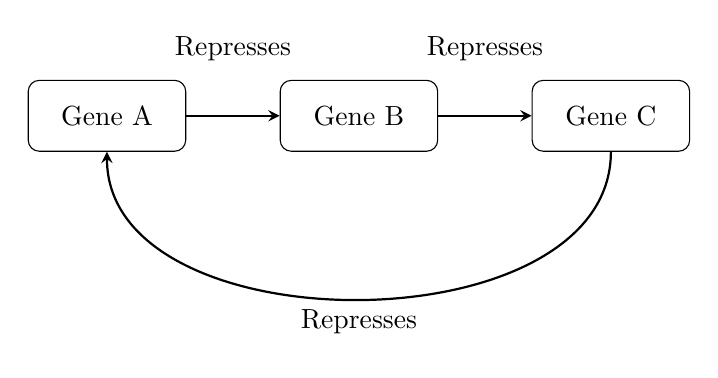
\begin{tikzpicture}[>=stealth, node distance=1.6cm]
\node[draw, rounded corners, minimum width=2.0cm, minimum height=0.9cm] (A) {Gene A};
\node[draw, rounded corners, minimum width=2.0cm, minimum height=0.9cm, right of=A, node distance=3.2cm] (B) {Gene B};
\node[draw, rounded corners, minimum width=2.0cm, minimum height=0.9cm, right of=B, node distance=3.2cm] (C) {Gene C};
\draw[->, thick] (A) -- (B) node[midway, above=16pt]{Represses};
\draw[->, thick] (B) -- (C) node[midway, above=16pt]{Represses};
\draw[->, thick] (C.south) to[out=270, in=270] node[midway, below]{Represses} (A.south);
\end{tikzpicture}
\end{center}

Mutual repression prevents settling: high A lowers B, low B raises C, and high C lowers A, repeating the cycle. Boxes and arrows aid thought; cells contain no actual wires.

Third, engineered microbes execute designed pathways as living chemical factories. Artemisinin is a particularly elegant example. This antimalarial originally came from sweet wormwood, with harvests dependent on weather. Scientists assembled wormwood and yeast genes in baker's yeast to produce artemisinic acid in tanks, followed by one chemical conversion to artemisinin. Chapter 83's recombinant insulin follows the same principle: \textbf{cells are factories; genes are production-line blueprints}. More ambitious teams write chromosomes from scratch. The international Synthetic Yeast Genome Project chemically synthesizes chromosomes and replaces natural versions, with cells remaining alive. Life's machinery is moving from readable and editable to writable.

\begin{tiaozhan}
Why must engineered bacteria remain contained in tanks? Under ideal conditions, E. coli divides about every twenty minutes. One cell undergoes 72 generations in 24 hours, theoretically yielding $2^{72} \approx 4.7\times 10^{21}$ cells. At about $10^{-12}$ grams each, the total is roughly $4.7\times 10^{9}$ kilograms, over four million tons, exceeding a day's global food production. Nutrients of course run out long before this, but the estimate illustrates \textbf{microbes' formidable exponential growth and the lack of an undo button after engineered traits escape}. Synthetic biology therefore adds safeguards: dependence on artificial nutrients absent from nature, causing starvation outside the factory, or kill switches responding to particular signals. Skipping the arithmetic is fine, but it explains why biosafety is not needless worry.
\end{tiaozhan}

\section{Biosafety: Escape, Misuse, and Oversight}

The final questions extend beyond individual products into ecology and society:

\begin{itemize}[itemsep=2pt]
\item \textbf{Ecological escape}. Outcomes depend on context. Virus-resistant Hawaiian papaya lacks cross-compatible wild relatives, lowering escape risk; herbicide-resistance transfer has occurred where compatible weeds grow nearby. Assess local relatives and the trait's survival advantage, applying individual evaluation at ecosystem scale. Gene drives push the issue further: CRISPR can raise transmission near $100\%$ rather than fifty-fifty, potentially spreading malaria-blocking traits through wild mosquitoes. Public-health benefits may accompany unpredictable, nearly irreversible ecological effects. Current consensus therefore favors strict laboratory containment first, with field release requiring case-specific assessment and international consultation.
\item \textbf{Dual use}. Tools for reading and writing DNA can make vaccines or dangerous pathogens; synthesizing known viruses is already possible. The response is oversight at key points, not suppressing science: synthesis-order screening, tiered laboratory controls, and international conventions.
\item \textbf{Benefits and burdens}. Seed patents and seed-saving rights, affordability, and who pays for long-term ecological monitoring are not chemical questions, but shape technology's outcomes. Science addresses feasibility and consequences; society must decide what should be done.
\end{itemize}

\section{Where This Assessment Framework Has Limits}

Product-by-product assessment has boundaries. First, genes and traits do not correspond one-to-one: pleiotropy means one change can have unexpected effects, requiring monitoring beyond short-term testing and commercialization. Second, editing may act off target (Chapter 82), requiring individual sequence verification. Third, complex ecosystems may reveal effects only after years at large scales, so absolute long-term safety promises exceed evidence. Conversely, permanent blanket prohibition also exceeds evidence. The honest stance is: \textbf{let policy follow evidence, testing as we proceed}.

\section{Back to the Papaya and Glowing Fish}

Now to answer our opening questions.

What happens to the papaya's viral coat gene after eating? Like billions of gene fragments in rice and pork, digestive enzymes break it into nucleotides, mostly absorbed, degraded, or excreted. Your cells lack a mechanism for picking up foreign DNA and installing it in their genome. Chapter 82 showed that even bacterial DNA uptake requires artificially created stringent conditions. Moreover, ordinary papaya can expose you to more complete viral particles. The answer is no, derived from digestion and absorption, not a natural-is-good slogan.

What about the fish? Their jellyfish fluorescent protein is harmless to people, but wild release may introduce competition and new genes. The issue lies in an introduced species, not fluorescence, much like released red-eared sliders, a network Chapter 86 revisits. The answer is do not release them, again following case-specific analysis.

\textbf{Translator safety note:} Never release aquarium fish or other pets into waterways, whether engineered or not; arrange responsible rehoming instead. Do not treat the protein discussion as approval to eat ornamental animals. See \href{https://www.fws.gov/story/dont-let-it-loose}{U.S. Fish and Wildlife Service release-prevention guidance}.

This chapter offers questions, not a list of pro- or anti-technology positions. Next we apply them to you: if a genetic report says a disease risk is $30\%$ higher, how can you understand it without unnecessary fear?

\section*{Try It Yourself}

\begin{sikaoti}
\item Draw the information flow from the viral coat gene in resistant papaya through transcription and translation to resistance, labeling each arrow. State that this depicts information, not a realistic cell.
\item Explain to an older relative convinced crossbreeding is naturally safe and transgenesis always dangerous why the number of changed genes is not a reliable risk measure. Include mutation breeding and its mutation scale.
\item Someone proposes introducing herbicide resistance into oilseed rape for local cultivation. List at least four specific assessment questions covering genes, proteins, dose, pollen movement, and local relatives.
\item Dolly's entire genome came from the nuclear donor, but her food, illnesses, and care were her own. Draw one score giving two performances to explain identical genomes with different traits and identify the sources of difference.
\item Starting with one E. coli dividing every twenty minutes, how many cells theoretically exist after ten hours? Express the result as a power of two and an order of magnitude in ten. If nutrients permit only one gram of biomass, when does growth brake? What limits microbes in tanks and nature?
\item Identical twins are called natural clones here. Design an observational test of whether identical genomes mean identical personalities. Who would you compare, and what confounders must you address?
\end{sikaoti}
